\section{Introduction}
\label{sec:introduction}

The graph is a fundamental abstraction for modeling relationships and 
dependencies across diverse domains, including social and information 
networks, transportation systems, cybersecurity provenance, and software 
package ecosystems~\cite{mislove2007measurement, leskovec2005graphs, 
kikas2017structure}. 
Among these, directed graphs 
% (digraphs)
are of particular interest 
as they capture asymmetric dependencies and causal flows that 
underpin critical analytics, such as breadth-first search (BFS)~\cite{lee1961algorithm}
%\YJ{add a citation for BFS, and later for SSSP and APSP} 
for traversal, single-source and all-pairs shortest paths (SSSP/APSP)~\cite{thorup1997undirected, seidel1992all}  for routing and dependency, and betweenness 
centrality (BC)~\cite{Brandes2001BC} for node importance.


Over the past years, graph processing systems and domain-specific 
frameworks have achieved substantial performance improvements for 
\emph{static} graph analytics on both CPUs and 
GPUs~\cite{Shun2013Ligra,Wang2016Gunrock,Zhang2018GraphIt}. 
% In parallel,  dynamic graph data structures have made it possible to ingest and  maintain evolving graphs under high update  rates~\cite{ediger2012stinger,Busato2018Hornet,Awad2020DynamicGPU}.
However, in many real-world domains, graphs are \emph{dynamic}, i.e., vertices and edges
continuously appear and disappear as the underlying system evolves~\cite{besta2021practice}. At the
same time, the users might issue \emph{ad hoc} queries with changing sources,
targets, and scopes. For example, a user may need to trace the blast
radius (i.e., the set of downstream services affected by a failure) of a newly
disclosed vulnerability, recompute reachability after
integrating new services, or update dependency analysis in an evolving
software ecosystem~\cite{brank2003download}. These traversal-centric tasks all
depend on the current graph structure and must be repeated as the graph evolves. These 
workloads combine continuous structural updates with repeated, query-driven 
traversals, forming an end-to-end pipeline that must be efficient in both 
dimensions.

Existing dynamic graph systems primarily focus on \textit{update throughput}, 
i.e., how quickly structural changes can be incorporated into the 
graph~\cite{ediger2012stinger,Busato2018Hornet,Awad2020DynamicGPU,fan2025cuckoograph}. 
However, update throughput only addresses part of the end-to-end workload. 
That is, after each structural change, downstream analytics such as BFS, SSSP, BC, 
and reachability often need to be recomputed, either partially or entirely. 
As graphs grow to billions of edges, such downstream graph analytics
% traversal-based algorithms 
increasingly dominate the total runtime. 
% In our experiments, downstream computation accounts for over $42.4\%$ \YJ{TODO\CQ{Done}}\CQ{42.4\% = downsteam time/ (downsteam time + building time)} of end-to-end execution time on large graphs~\cite{Hanauer2022DynSurvey}. 
Therefore, optimizing update throughput alone is not enough, while reducing the cost of downstream graph computation under 
continuous evolution is equally critical.

% Graphs provide a natural abstraction for modeling relationships and dependencies in domains such as social and information networks, transportation systems, cybersecurity provenance, and software package ecosystems~\cite{rahman2025hugginggraph, brank2003download,kikas2017structure}. 
% Directed graphs (digraphs) capture asymmetric dependencies and causal flows, which underpin fundamental analytics including breadth-first search (BFS), single-source and all-pairs shortest paths (SSSP/APSP), and betweenness centrality (BC)~\cite{Brandes2001BC}. 
% Over the past decade, graph processing systems and domain-specific frameworks have achieved substantial performance improvements for \emph{static} graph analytics on both CPUs and GPUs~\cite{Shun2013Ligra,Wang2016Gunrock,Zhang2018GraphIt}. 
% In parallel, dynamic graph data structures have made it possible to ingest and maintain evolving graphs under high update rates~\cite{Ediger2012Stinger,Busato2018Hornet,Awad2020DynamicGPU}.
% However, real-world graphs are not only \emph{large} but also inherently \emph{dynamic}. 
% Vertices and edges continuously appear and disappear, while analysts issue \emph{ad hoc} queries with changing sources, targets, and scopes. 
% For example, analysts may need to trace the blast radius of a newly disclosed vulnerability, recompute reachability after integrating new services, or update dependency analysis in evolving software ecosystems. %cite here

% Existing dynamic graph systems primarily focus on \textit{update throughput}, i.e., how quickly structural changes can be incorporated into the graph~\cite{Ediger2012Stinger,Busato2018Hornet,Awad2020DynamicGPU}. 



% While high update throughput is essential, it addresses only part of the end-to-end workload. 
% After each structural change, downstream analytics, such as BFS, SSSP, BC, and reachability, often need to be recomputed either partially or entirely. 
% As a result, in practical deployments, dynamic updates and downstream graph algorithms together form the end-to-end processing pipeline and frequently become the dominant computational bottleneck~\cite{Hanauer2022DynSurvey}. 
% In other words, optimizing updates alone is insufficient; the efficiency of downstream graph computation under continuous evolution is equally critical.

% \subsection{Motivation}
% \subsection{Two Extremes of Reusing Prior Computation}


% \begin{figure}[t]
%     \centering
%     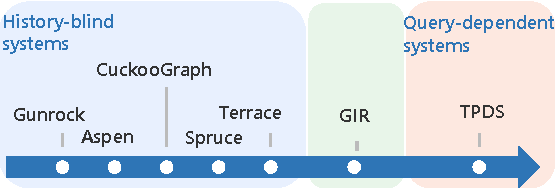
\includegraphics[width=\linewidth]{figures/history_blind-crop.pdf}
%     \caption{Dynamic graph systems classified by their use of prior
%     computation for downstream analytics.
%     History-blind systems (left) discard all prior results after each
%     update.
%     Query-dependent systems (right) cache results for a specific
%     query and source.
%     GIR (center) maintains query-agnostic structural invariants that
%     benefit all downstream algorithms.\YJ{Polish figure and caption to match this description. \CQ{Done}}}
%     \label{fig:history_query}
% \end{figure}

\textbf{Two extremes of reusing prior computation.} After a graph update, the results from previous computation do not 
simply become invalid.
Consider running SSSP from source $s$ on graph snapshot $G$,
when $G$ is updated to $G'$, many of the shortest paths from $s$ 
remain unchanged.
A system that could identify which results are still valid and which 
need to be recomputed would avoid a large fraction of redundant work.
However, the key question is, in what form should prior computation be retained to maximize reuse?
% As illustrated in Fig.~\ref{fig:history_query}, 
% Unfortunately, 
Existing approaches fall into two extremes, where they either igore such previous computation information (history-blind system) or overly rely on them (query-dependent system). 
% is well suited for ad hoc dynamic graph workloads.
% Particulalry,

\textit{(i) History-blind systems.}
Most dynamic graph systems, including Terrace~\cite{pandey2021terrace}, 
Spruce~\cite{shi2024spruce}, and Aspen~\cite{dhulipala2019low}, treat each query independently.
That is, after an update, such a system integrates the change into the graph representation and reruns the queried graph algorithm.
These systems are generic to any queries, while they discard the 
prior computation after every update.
For large graphs with frequent updates, such a system will incur large overhead due to repeated recomputation.
% is the dominant source of overhead.
% ~\cite{ramalingam1996computational}.

\textit{(ii) Query-dependent systems.}
A different class of systems try to reuse prior results more
directly.
For example,
% \textit{Khanda et al.}~\cite{khanda2021parallel} maintain an SSSP tree rooted at a fixed source $s$ after each query~\cite{khanda2021parallel}.
\textit{Khanda et al.} designed a method by maintaining  
% TPDS\cite{khanda2021parallel} maintains 
an SSSP tree rooted 
at a fixed source $s$~\cite{khanda2021parallel}.
\cq{Upon an update, they recompute only the affected subtree.
\textit{GraphBolt}~\cite{mariappan2019graphbolt} and
\textit{DZiG}~\cite{mariappan2021dzig} maintain per-vertex aggregation
dependencies for a fixed algorithm (e.g., PageRank) and propagate only the
incremental delta caused by mutations.
\textit{Kickstarter}~\cite{vora2017kickstarter} retains approximate monotonic results for path-based algorithms and propagates corrections after updates.
These approaches can be efficient when the same algorithm is repeated on the same graph.
However, they are tied to specific queries, e.g., a specific source vertex for SSSP query.
% However, each system is tied to a specific algorithm and, in some cases, a specific source vertex.
If the next query uses a different source, or switches to a different algorithm,
the cached state provides no benefit and must be rebuilt.}
In practice, dynamic graph workloads are dominated by \emph{ad hoc} queries
with varying sources, targets, and algorithms~\cite{Hanauer2022DynSurvey}.
Thus, such query-dependent systems offer limited reuse in practice.



% One natural way to reduce downstream recomputation is to retain and
% exploit the \emph{history of structural changes}.
% When an edge is inserted or deleted, not all downstream algorithms are
% equally affected.
% Only those that depend on the connectivity region touched by the update
% need to be re-executed.
% If a system could identify which structural invariants changed and which
% did not, downstream algorithms could skip unaffected regions entirely,
% rather than recomputing from scratch after every update.


% Modern applications increasingly rely on dynamic graphs, where edges and vertices evolve continuously over time. 
% Beyond the current snapshot, the \emph{history of updates} is essential for temporal reasoning, incremental computation, 
% and maintaining structural properties. However, existing systems treat history as either transient streams or low-level 
% storage artifacts, rather than a first-class abstraction for structural computation.



% As illustrated in Fig.~\ref{fig:history_query}, prior systems utilize history at different levels. 
% Streaming systems such as Terrace and Spruce process updates in an ephemeral manner, without retaining history for 
% structural reasoning. In contrast, systems like Aspen support versioned snapshots via persistent data structures, 
% enabling access to past states. However, such history remains at the data level and does not capture the evolution of 
% higher-level structures (e.g., SCCs or BCTs), leading to costly recomputation under updates.

% The key limitation is that \emph{history is stored but not understood}. Existing approaches fail to capture the semantic 
% impact of updates on graph structure, which is critical for connectivity-centric tasks.

% \textbf{A Compiler Mindset for Dynamic Graph}
% \subsection{A Compiler Mindset for Dynamic Graph}

\textbf{A compiler mindset for dynamic graph}.
The two extremes reveal a clear gap.
That is, we need a method that not only leverages historical computation results but also is not tied to any specific queries or algorithms.
% What is needed is a form of 
% prior computation that is incrementally maintained across updates and is not tied to any specific query or source.
% To address this gap, 
Inspired by the intermediate representation (IR) design in compiler~\cite{Lattner2004LLVM}, we propose a new  IR for dynamic graphs, named graph IR (GIR).
The goal is to capture \textbf{\textit{reusable structural invariants}} that persist across dynamic updates and can benefit many algorithms, without being tied to any specific queries or algorithms.

Just as a compiler IR sits between front-end parsing and back-end optimization passes, GIR sits between graph updates and downstream analytics.
% \YJ{working on}
As shown in Figure~\ref{fig:gir_ir}, this mirrors the compiler
pipeline. That is, updates modify the graph structure (analogous to front-end), 
and downstream algorithms repeatedly operate on the result
(analogous to optimizations).


% To address this, we propose a \emph{Graph Intermediate Representation (GIR)} that elevates history to a 
% \emph{structure-aware abstraction}. GIR maintains a compressed history that encodes structural evolution, enabling 
% efficient incremental updates across multi-granular connectivity representations. Instead of recomputing from scratch 
% or replaying full histories, GIR localizes changes and propagates updates efficiently across hierarchical structures.

% \YJ{Need more discussions on dynamic graph algorithm computation.}

% \textbf{Dynamic graph algorithm computation in practice.}
% Although theoretical research has proposed sophisticated fully dynamic algorithms for reachability, connectivity, and shortest paths~\cite{King1999TransitiveClosure,Demetrescu2004DynamicAPSP}, as well as incremental techniques for SSSP and centrality~\cite{Ramalingam1996Incremental,Nasre2014IncBC}, bridging theory and practical systems remains challenging.
% First, many dynamic algorithms assume fixed sources or specific query patterns, whereas real workloads are dominated by \emph{ad hoc} queries with changing sources and scopes~\cite{Hanauer2022DynSurvey}.
% Second, deletions and structural churn may trigger complex dependency updates, leading to high worst-case repair costs.
% %Third, modern parallel hardware such as GPUs favors regular, bulk-synchronous execution, while dynamic maintenance often introduces irregular control flow and scattered memory accesses~\cite{Gao2024DynGPUSurvey}.
% We also observe that as graph size grows, downstream computation increasingly dominates overall runtime.
% For smaller graphs, update processing and downstream analytics contribute comparable costs.
% However, for larger graphs, traversal-based algorithms such as BFS, SSSP, and BC account for the majority of execution time.
% This observation suggests that optimizing update throughput alone is insufficient for improving the performance of dynamic graph systems.
% Consequently, even when update throughput is high, downstream graph algorithms still incur substantial recomputation overhead under continuous evolution.
% Instead, reducing the cost of downstream analytics is critical for achieving scalable end-to-end performance.


%\YJ{Need two types of numbers (better to be in a figure), 1. +how slow are the downstream graph algorithms. 2. how slow are the end-to-end computation.}

% \textbf{A compiler mindset for dynamic graphs.}
% In compiler design, an intermediate representation (IR) separates front-end parsing from back-end optimization, enabling multiple optimization passes without repeatedly analyzing the original source code~\cite{Lattner2004LLVM}. 
% We observe a similar separation in dynamic graph processing: dynamic updates continuously modify the graph structure (analogous to parsing), while downstream algorithms repeatedly operate on the evolving graph (analogous to optimization passes).
% Motivated by this perspective, we introduce the \textbf{Graph Intermediate Representation (GIR)}, a dynamic and query-agnostic representation that persists across updates and exposes reusable structural invariants for downstream analytics.
% \YJ{Add a figure to show the connection between IR and GIR.}


% GIR is guided by three design principles. 
% (i) First, the invariants must be \textit{algorithm-independent}, capturing structural properties that benefit many graph algorithms rather than any single one. 
% (ii) Second, they must be \textit{incrementally maintainable}, allowing each invariant to be repaired after a local graph update without full recomputation. 
% (iii) Third, they must be \textit{multi-granular}, collectively exposing graph structure at multiple levels, from global connectivity down to local articulation boundaries. so that algorithms can prune their search space at whichever level is most appropriate.

% GIR is guided by three design principles.
% (i) First, the invariants must be \emph{algorithm-independent}: they should capture structural properties
% that benefit many graph algorithms, not just one.
% (ii) Second, they must be \emph{incrementally maintainable}: each invariant should be repairable
% after a local graph update without a full recomputation.
% (iii) Third, they must be \emph{multi-granular}: together, they should expose graph structure
% at multiple levels, from global connectivity down to local articulation boundaries,
% so that algorithms can prune their search space at whichever level is appropriate.

% However, this GIR needs to be efficient for under dynamic workloads, which poses three key
% challenges.
% \textbf{(i)} \textit{High update velocity} requires low-latency structural
% repair after each edge insertion or
% deletion.
% \textbf{(ii)} It can handle \textit{ad hoc queries} that the query source and type
% change frequently.
% \textbf{(iii)} \textit{scale and skew}, where billion-edge graphs with
% heavy-tailed degree distributions stress memory locality and load
% balancing on multi-core and GPU
% systems.
% To address these challenges, GIR enforces strict scope control.
% Each update triggers only the minimal structural repairs necessary,
% preventing maintenance overhead from outweighing the gains in
% downstream performance.

%\begin{figure}[t] % \centering % 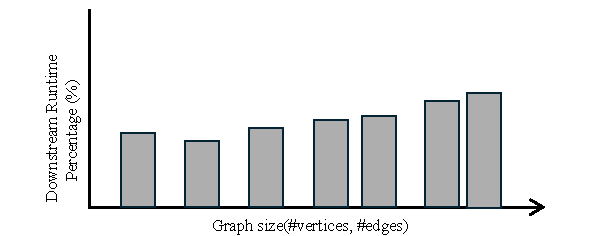
\includegraphics[width=\linewidth]{figures/Presentation2.pdf} %\caption{ %\textbf{Downstream computation increasingly dominates end-to-end runtime as graph size grows.} %The figure shows the percentage of runtime spent in downstream graph algorithms (e.g., BFS, SSSP, BC) relative to the total end-to-end processing time. %As the graph size increases, downstream computation becomes the dominant cost in the dynamic graph processing pipeline. %This trend highlights the importance of optimizing downstream analytics rather than focusing solely on update throughput. %\YJ{TODO} %} % \Description{Figure description.} % \label{fig:downstream_ratio} %\end{figure} %Figure~\ref{fig:downstream_ratio} illustrates how the runtime distribution changes as graph size increases. %The figure reports the percentage of runtime spent in downstream graph algorithms relative to the total end-to-end processing time.



% \YJ{This can merge with the previous paragraph. No need to discuss our concrete design of GIR at this stage.}

% Rather than caching answers for specific sources or queries, GIR maintains multi-granular connectivity structures—such as connected components (CC), strongly connected components (SCC) and their condensation DAG, and biconnected components (BiCC)—because these invariants provide algorithm-independent \emph{boundaries} and \emph{jump points}.
% These structural boundaries localize the impact of updates and allow traversal-based analytics to skip unaffected regions or shortcut exploration across certified structural cuts.
% \YJ{@YJ, needs further polishing.} \YJ{Challenges:
% Challenge 1. Inefficient graph update --> GIR;
% Challenge 2. Limited parallelism --> Concurrent computation framework} 

% Maintaining such structural information is challenging under three key properties of modern workloads:
% (i) \textbf{High update velocity}, which requires low-latency maintenance~\cite{Ediger2012Stinger,Busato2018Hornet};
% (ii) \textbf{Ad hoc queries}, which limit the effectiveness of source-specific caching~\cite{Hanauer2022DynSurvey};
% and (iii) \textbf{Scale and skew}, where billion-edge graphs with heavy-tailed degree distributions stress memory locality and load balancing on both CPUs and GPUs~\cite{Shun2013Ligra,Wang2016Gunrock,Zhang2018GraphIt,Gao2024DynGPUSurvey}.
% To prevent maintenance overhead from overwhelming query gains, our GIR also enforce strict \emph{scope control}, ensuring that each update triggers only the minimal necessary repairs.

% \subsection{Contribution}
% \label{subsec:contribution}

\begin{figure}[t]
    \centering
     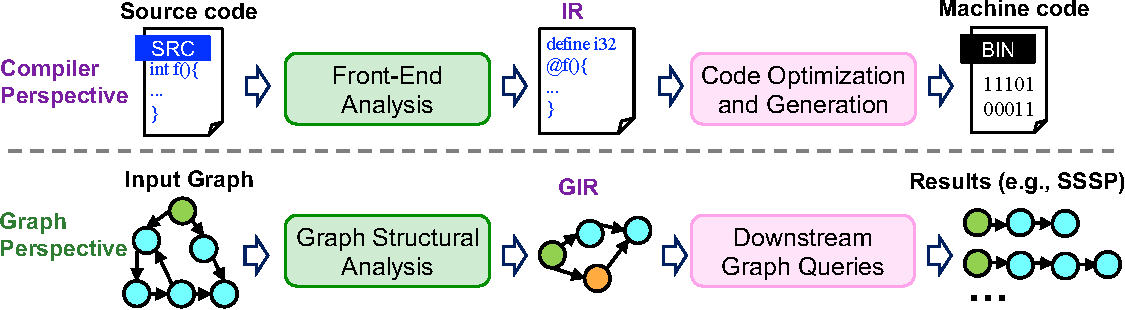
\includegraphics[width=1\linewidth]{figures/compiler_figure.pdf}
    \caption{\textit{From compiler IR to Graph IR (GIR).}
    Compiler IR enables reusable optimizations across different programming languages. Similarly, GIR maintains reusable structural invariants across dynamic updates.}
    \label{fig:gir_ir}
\end{figure}

% Particularly, this paper makes three major contributions.

\textbf{Contribution}.
Building GIR under continuous, high-velocity updates with ad hoc query patterns is nontrivial.
There are three challenges must be addressed.
\emph{(i) Update velocity}: low-latency GIR repair is required after each node/edge insertion or deletion.
\emph{(ii) Ad hoc queries}: the query source, target, and algorithm can change between requests. Thus, no query-specific state can be assumed.
\emph{(iii) Large scale graphs}: the graph could become large, e.g., with billion edges. Thus, the end-to-end computaiton, including update and query, needs to be efficient.
% sheer size of billion-edge graphs places sustained pressure on memory locality and makes efficient load balancing increasingly difficult on multi-core systems.
% \emph{(iii) Scale and skew}: billion-edge graphs with heavy-tailed degree distributions stress memory locality and load balancing on multi-core systems.
To address such challenges, this paper presents GIR, a scalable dynamic graph analytics system based on a newly designed persistent intermediate representation. Particularly, we make four major contributions.

% \textbf{Graph intermediate representation (GIR).}
% We devise GIR, a dynamic and query-agnostic structural layer for dynamic graphs.
% Particularly, the GIR integrates three fundamental structural algorithms. 
% \YJ{Why designing in this way.}
% First, \emph{weakly connected components (WCCs)} partition the graph into independent regions, which allow  downstream algorithms immediately skip entire components that are unreachable from a query source, pruning the largest unnecessary work at the coarsest level.
% Then, \emph{strongly connected components (SCCs) and their condensation directed acyclic craph (DAG)} capture directed
% reachability and cycle structure within each WCC.
% The condensation DAG reduces directed traversal to a DAG walk, eliminating redundant exploration of cyclic subgraphs.
% \emph{Biconnected components (BiCCs) and their block-cut tree (BCT)} expose articulation
% boundaries within each SCC.
% The BCT reveals which subgraphs are structurally independent, allowing algorithms to
% process each block separately without crossing unnecessary cut vertices.
% These algorithms are chosen because they are algorithm-independent structural invariants. They expose natural boundaries and hierarchical structure that many algorithms implicitly rediscover during computation.

\textbf{Graph intermediate representation (GIR).}
We devise GIR, a dynamic, query-agnostic structural layer for graphs. GIR integrates three fundamental primitives. First, \emph{weakly connected components (WCCs)} partition the graph into independent regions, enabling algorithms to skip unreachable components and prune work at a coarse level. Second, \emph{strongly connected components (SCCs)} and their condensation directed acyclic graph (DAG) capture directed reachability, reducing traversal to a DAG and avoiding redundant exploration of cycles. Third, \emph{biconnected components (BiCCs)} and the block-cut tree expose articulation boundaries, allowing independent processing of subgraphs. 
% These primitives are algorithm-agnostic structural invariants that reveal natural boundaries and hierarchy often rediscovered during computation.
These three primitives are chosen because they are algorithm-independent structural invariants that expose natural hierarchical boundaries many algorithms implicitly rediscover during computation.

\textbf{Structure-aware incremental maintenance.} We design an incremental maintenance method that keeps GIR structurally consistent under dynamic graph updates without full recomputation. 
\textit{The core insight is that GIR's three-layer hierarchy enables a metadata-only classification of every edge insertion or deletion into one of five structurally distinct cases, each confining repair to the minimum necessary region.}
We formalize this as a scope-prune-update strategy for single-edge updates and extend it to a filter-merge-update strategy for batch updates. 
Together, they eliminate redundant operations, merge overlapping maintenance regions, and enable parallel execution.
% across independent regions. 
% Together, they eliminate redundant operations, merge overlapping maintenance regions, and enable parallel execution across independent regions. 
% Compared to recent methods on dynamic graph computation, 
Benefited from this, for the update with both insertions and deletions, on all the tested graphs, GIR achieves an average throuput of $25.4$ million edges per second (MEPS), which is $1.8\times$ more than state-of-the-art methods.
% achieves an average of $8.5\times$, $1.9\times$, and $1.8\times$ speedup for update throughput over recent methods, including Spruce, Terrace, and Aspen, respectively.
%citation here

% On seven real-world graphs, GIR achieves 
% $8.5\times$ over Spruce, $1.9\times$ over Terrace, and $1.8\times$ over Aspen.
% average mixed-update throughput speedups of $8.5\times$ over Spruce, $1.9\times$ over Terrace, and $1.8\times$ over Aspen.
% Evaluated on seven real-world graphs, GIR achieves average mixed-update throughput speedups of $8.5\times$ over Spruce, $1.9\times$ over Terrace, and $1.8\times$ over Aspen.
%\YJ{Any benefit numbers? Like, how much throughput improvement?}
% Together, SPU and FMU provide correctness and efficiency guarantees that no flat or single-layer index can match.

% \textbf{Cascading repair ...}
% To maintain GIR efficiently, we develop the \emph{Scope-Prune-Update} strategy.
% SPU first identifies which structural layers are affected by an update, then restricts
% repair to the smallest affected region, and finally performs localized structural fixes.
% For batch updates, we extend SPU into the \emph{Filter-Merge-Update} pipeline,
% which removes redundant operations, groups related updates by affected region, and
% processes them in parallel.
% To the best of our knowledge, GIR is the first dynamic, query-agnostic intermediate
% representation that maintains multi-granular connectivity structures for reuse
% across downstream graph algorithms.
% including 
% weakly connected components (WCCs), strongly connected components
% (SCCs) and biconnected components (BiCCs).
% These invariants are algorithm-independent.
% They expose natural structural boundaries that traversal-based
% algorithms implicitly rediscover on every query.
% By keeping these boundaries explicit and up to date, GIR allows
% downstream algorithms to skip unaffected regions and shortcut
% traversal across structural cuts.
% The same GIR can accelerate BFS, SSSP, betweenness centrality, and
% reachability queries, without any query-specific precomputation.
% % GIR maintains WCCs, SCCs and their condensation DAG, and BiCCs
% % organized as block-cut trees, incrementally under continuous updates.
% % These invariants are reused across diverse downstream analytics,
% % avoiding redundant recomputation.
% To maintain GIR efficiently, we develop the {Scope-Prune-Update
% (SPU)} strategy.
% SPU first identifies which structural layers are affected by an
% update, then restricts repair to the smallest affected region, and
% finally performs localized structural fixes.
% This ensures that each update triggers only the minimal necessary
% work.
% For batch updates, we extend SPU into the {Filter-Merge-Update
% (FMU)} pipeline, which removes redundant operations, groups related
% updates by affected region, and processes them in parallel.
% To the best of our knowledge, GIR is the first dynamic,
% query-agnostic intermediate representation that maintains
% multi-granular connectivity structures for reuse across downstream
% graph algorithms.

\textbf{GIR-enabled two-level parallel execution.}
Conventional dynamic graph systems rely primarily on data parallelism,
% ~\cite{ediger2012stinger,Busato2018Hornet,Awad2020DynamicGPU,fan2025cuckoograph}, 
i.e., all threads work
on the same task simultaneously.
GIR unlocks a second, complementary form of parallelism, i.e., task parallelism.
As GIR explicitly decomposes the graph into independent structural units, multiple
units can be processed as concurrent tasks, each without inter-task synchronization.
% Taking BFS and SSSP as examples, 
% For BFS and SSSP, 
Taking BFS as an example,
we can prune their search space using the condensation DAG and then execute one task per BiCC block in parallel.
% For DFS, which is traditionally sequential and difficult to parallelize on flat graphs\cite{malumbres2000efficient},
% BiCC blocks provide naturally independent subtasks, making DFS parallelizable for the first time in a practical setting.
%\YJ{64 or 128?}
% Particularly, with 64 threads, our method achieves average $1.9\times$ task-level speedup over conventional graph execution on large graphs, including livejournal, twitter and friendster, by running BFS. 
% Particularly, on the tested graphs, GIR achieves an average of $3\times$, $1.3\times$, and $1.3\times$ speedup for running BFS over Spruce, Terrace, and Aspen, respectively. 
With the additional task parallelism, 
% Benefited from this, 
on all the tested graphs, GIR achieves an average of $1.2\times$, $1.2\times$, and $1.7\times$ speedups over state-of-the-art methods for running BFS, SSSP, and betweenness centrality (BC), respectively.
% $1.3- 3\times$ average speedups for BFS over state-of-the-art methods.
% besides BFS, on SSSP acheives $2.7\times$ average speedups,
% BC acheieves $1.7\times$ everage speedups by comparing with state-of-the-art methods


% \YJ{TODO}


% \YJ{TODO}
%\YJ{Be specific. Which graphs? Which compared methods?}
%\YJ{Fill in concrete numbers.\CQ{Done}}




\textbf{End-to-end evaluation.}
%update throughput
We evaluate GIR on seven real-world graphs covering social networks,
citation graphs, and web graphs, with the largest one having $2.4$ billion edges.
\cq{We compare GIR against state-of-the-art dynamic graph computation methods, i.e., Terrace~\cite{pandey2021terrace}, Aspen~\cite{dhulipala2019low}, and Spruce~\cite{shi2024spruce} for update throughput and BFS/BC analytics, and additionally against GraphBolt~\cite{mariappan2019graphbolt} and DZiG~\cite{mariappan2021dzig} for BFS/SSSP analytics.}
For update throughput,
on average, GIR achieves $22.6$ MEPS for \textit{insertion-only update}, which is $9.1\times$, $3.4\times$, and $2.7\times$ more than Spruce, Aspen, and Terrace, respectively. 
For \textit{deletion-only update}, GIR achieves $8.5\times$, $4.4\times$, $3.4\times$ over Spruce, Aspen, and Terrace, respectively. 
\cq{For downstream graph analytics, GIR achieves average speedups of $1.6\times$ on BFS over Spruce, Terrace, Aspen, GraphBolt, and DZiG.
% (up to $3\times$ over Spruce on structured graphs); 
% For SSSP, GIR achieves $2.7\times$ over Spruce, $1.6\times$ over DZiG, and $1.2\times$ over GraphBolt; 
For SSSP, GIR achieves $2.7\times$, $1.6\times$, and $1.2\times$ over Spruce, DZiG, and GraphBolt, respectively.
For BC, GIR achieves $1.7\times$ over Terrace and Aspen.}
In addition, GIR shows strong and stable scalability across all tested datasets.
% In addition, GIR shows strong and stable scalability, achieving $20.9\times$ average speedup at 64 threads, ahead of Spruce ($17\times$).
% on average, GIR achieves $22.6$ MEPS for \textit{insertion-only} updates ($9.1\times$, $3.4\times$, and $2.7\times$ over Spruce, Aspen, and Terrace) and $8.5\times$, $4.4\times$, $3.4\times$ more for \textit{deletion-only} updates.
% $9.1\times$, $3.4\times$, and $2.7\times$ more than Spruce, Aspen, and Terrace, respectively.
% \cq{For downstream graph analytics, GIR achieves average speedups of $1.3\times$ on BFS over Spruce, Terrace, Aspen, GraphBolt, and DZiG (up to $3\times$ over Spruce on structured graphs); 
% $2.7\times$ on SSSP over Spruce, $1.6\times$ over DZiG, and $1.2\times$ over GraphBolt; and $1.7\times$ on betweenness centrality over Terrace and Aspen.}
% In addition, GIR shows strong and stable scalability, achieving $20.9\times$ average speedup at 64 threads, ahead of Spruce ($17\times$).



%We compared GIR with state-of-the-art dynamic graph computation methods, including Terrace~\cite{pandey2021terrace}, Aspen~\cite{dhulipala2019low}, and Spruce~\cite{shi2024spruce}.
%\YJ{Two aspects, (1) update throuput; (2) performance on graph algorithms.}
%Besides the mixed (insertion and deletion update), 
% Specifically,or \textit{insertion update},
%on average, GIR achieves $22.6$ MEPS for \textit{insertion-only update}, which is $9.1\times$, $3.4\times$, and $2.7\times$ more than Spruce, Aspen, and Terrace, respectively. 
%For \textit{deletion-only update}, GIR achieves $8.5\times$, $4.4\times$, $3.4\times$ more than Spruce, Aspen, and Terrace, respectively. 
%for insersion-only updates, we achieve average $5.0\times$,  speedup $9.1\times$ over Spruce, $3.4\times$ over Aspen, $2.7\times$ over Terrace,
%for deletion-only updates, we achieve $8.5\times$ over spruce, $4.4\times$ over Aspen, $3.4\times$ over Terrace
%our average throughput is 25.4 meps versus Aspen 14 meps, Terrace 13.6 meps Spruce 3 meps
% on mixed insertion/deletion workloads, GIR
% achieves average speedups of $8.5\times$ over Spruce, $1.9\times$ over
% Terrace, and $1.8\times$ over Aspen.
% (ii) For downstream \textit{graph analytics}, GIR achieves an average $3\times$ speedup on BFS over Spruce, $2.7\times$ on SSSP over Spruce, and $1.7\times$ on BC over both Terrace and Aspen.
% (iii) 
% \textit{Scalability}: 
%In addition, GIR shows strong scalability.
%\YJ{TODO}
%That is, with 64 threads, GIR achieves xx speedups 
%GIR scales to average $47\times$--$50\times$ speedup at 64 threads, %on large graphs (LJ and WT), 
% achieves $6.8/times$ speedup 
%consistently outperforming all baselines at every thread count.
%In addition, GIR shows strong and stable scalability across all tested datasets.
% On average GIR achieves $20.9\times$ speedup at 64 threads, ahead of Spruce ($17\times$).
% On graphs with many independent BiCC blocks (WT and LJ), GIR reaches $47.4\times$ and $45\times$ self-speedup at 64 threads, outperforming Spruce ($17.0\times$ and $45\times$) and Aspen ($43.6\times$ and $45\times$) on WT.
% On graphs with fewer blocks (WG and CP), GIR reaches $7.5\times$ and $11.0\times$ at 64 threads.
% On average across all datasets, GIR achieves $20.9\times$ speedup at 64 threads, ahead of Spruce ($17.0\times$).
% \YJ{TODO}


%\YJ{Also discuss scalability.}


% \YJ{Fill in numbers from experiment section.\CQ{Done}}

% \subsection{Contribution}

% \YJ{For each contribution, we need to add numbers.}

% % Here we summarize the key contributions of our GIR design.
% % \YJ{Then, briefly discuss the specific contributions. One per paragraph.}
% We make three major contributions.

% \textbf{Graph Intermediate Representation (GIR).}
% We introduce GIR, a reusable and query-agnostic graph representation that maintains structural invariants and lightweight summaries under continuous updates, enabling diverse ad hoc analytics to avoid redundant recomputation. GIR complements dynamic graph stores that prioritize update throughput~\cite{Ediger2012Stinger,Busato2018Hornet,Awad2020DynamicGPU} and static graph DSLs that optimize compute-only performance~\cite{Shun2013Ligra,Wang2016Gunrock,Zhang2018GraphIt}.
% Based on GIR, we further develop the SPU strategy, an incremental maintenance method that restricts structural repairs to a bounded region of influence in the condensation structure, thereby avoiding global recomputation.
% Rather than optimizing a single algorithm, GIR provides a reusable structural backbone that supports multiple analytics simultaneously, similar to how a compiler IR supports multiple optimization passes.
% Our goal is to enable a responsiveness-oriented dynamic graph processing pipeline in which both updates and downstream computation can execute efficiently.

% To the best of our knowledge, prior work has not introduced a dynamic, query-agnostic intermediate representation that maintains multi-granular connectivity structures for reuse across downstream algorithms.
% % This gap motivates the design of GIR.

% \textbf{GIR-Enabled Task Parallel Execution Framework.}
% We design traversal kernels for BFS, SSSP, BC and DFS that leverage GIR structural hints to prune unnecessary exploration and accelerate query execution.
% By exploiting the hierarchical structure exposed by GIR, the framework also enables effective parallelization.
% Even algorithms that are traditionally sequential, such as DFS, can benefit from the structural parallelism provided by our framework.
% \YJ{Add measurable benefit numbers. E.g., how much parallelism has been improved.}


% \textbf{End-to-end evaluation.}
% Through extensive experiments on real and synthetic dynamic workloads, we demonstrate substantial improvements in downstream latency and overall end-to-end responsiveness while maintaining competitive update throughput on modern multi-core systems.

% \YJ{Needs further polishing.}